\chapter{Drone Avionics}
\minitoc
\thispagestyle{plain}

\renewcommand{\arraystretch}{1.75}

In this chapter we explore the searching algorithm applied to a dynamic simulated device really close to our drone. The simulation will use a simpler control model (LQR) and will implement the perception action paradigm for the searching part. Searching part will be performed with device implemented in previous chapter, with auxiliary range finder for obstacle avoidance and altitude keeping. All those elements build what is called avionic framework of the drone. The basic idea is to create a stacked structure that could be easily expanded in future; again, what we are discussing in an initial platform that could be improved with the use of more increasingly complex sensor--fusion, that allows to exploit the most sophisticated searching algorithm possible. 

\section{Perception Action paradigm}
The perception--action (PA) paradigm has a very strict connection with the definition of our searching algorithm. Lets try to understand what this paradigm is.

\subsection{The basic paradigm}
A PA map consider an agent in which external stimuli derive from a sensor network, that perform the perception section of the agent. Perception is therefore translated into a symbol that could be handled by the action section of the agent.
\begin{figure}[h]
\caption{Classical percetion--action map}
\centering
\begin{tikzpicture}[auto, node distance=2cm,>=latex']
	\node[input] (input) {};
	\node[block,right of=input] (perception) {Perception};
	\node[block,right of=perception] (action) {Action};
	\node[output, right of=action] (output) {};

	\draw[->] (input) -- node[pos=0.2] {Sensors} (perception);
	\draw[->] (perception) -- (action);
	\draw[->] (action) -- node[pos=0.7] {Actuators} (output);
\end{tikzpicture}
\end{figure}

Making a straight example on our device: we consider as sensor elements our digital ARTVA; the input to the perception stage, should be analyzed to perform an action, that is the movement of the drone towards buried position.

The relationship between the agent and the environment is called \emph{situatedness}, while the intercourse within what represents the \emph{body} on what represents the \emph{mind} of the agent is called \emph{embodiment}, as explained in \citep{thedynamicsofactivecaterogicalperception}.
\begin{marginfigure}
\centering
\begin{tikzpicture}[auto, node distance=1cm,>=latex']
	\node [rectangle, draw=black, minimum width=5cm,minimum height=3cm] (envir) {};
	\node [rectangle, draw=black, minimum width=3cm,minimum height=2.25cm] (body) at ++(0.75cm,-0.25cm) {};
	\node [rectangle, draw=black, dashed, minimum width=1.5cm,minimum height=1.5cm] (body) at ++(1.25cm,-0.5cm) {};
	\node [rectangle, fill=white] (situatedness) at ++(-0.75cm,-0.65cm) {$\underset{situatedness}{\longleftrightarrow}$};
	\node [rectangle, fill=white] (embodiment) at ++(.5cm,-0.85cm) {$\underset{embodiment}{\longleftrightarrow}$};
	\node [rectangle, fill=white, draw=black] at ++(-1.25cm,1.5cm) {\textbf{Environment}};
	\node [rectangle, fill=white, draw=black] at ++(1.5cm,0.85cm) {\textbf{Agent}};
	\node at(-0.3cm,0.6cm) {Body};
	\node at(1cm,0cm) {Mind};
\end{tikzpicture}
\caption{Embodiment and situatedness}
\end{marginfigure}

\subsection{Exploiting more complex behavior}
\myparagraph{Expanding PA}
Apart the basic behavior, the advantages of PA maps are related too the implementation of extremely complex actions using other techniques such as:
\begin{itemize}
\item subsumption and grounding
\item innate knowledge
\item bootstrapping
\item historical knowledge
\item shared knowledge
\end{itemize}
All those element could be serially implemented, one after the other, while they run together to create a coherent attitude with respect to the problem. One of the advanced feature that we will use in this project is the subsumption and the grounding of the symbols.

\myparagraph{Subsumption and grounding}
The \emph{symbols grounding} is an implementation of the embodiment of the agent as a stacked architecture in which different layer (subsumption), that performs different operations, are piled up in such a way that higher level, of higher complexity, could transparently use lower levels (symbols grounding \citep{harnad1990symbolgrounding}), and incorporate them to reach more complex behavior.
\begin{marginfigure}
\begin{tikzpicture}[auto, node distance=2cm,>=latex']

	\matrix [draw=white, row sep=0.1cm, column sep=1.5cm] {	
	   	& \node [block, right, anchor=west, text width=1.5cm, minimum width=1.5cm] (levelD) {Level 3}; & \\
		& \node [block, right,anchor=west, text width=1.8cm, minimum width=1.8cm] (levelC) {Level 2}; & \\
	 	& \node [block, right,anchor=west, text width=2.1cm, minimum width=2.1cm] (levelB) {Level 1}; & \\
		\node [input,right] (input) {}; & \node [block,anchor=west, text width=2.4cm, right, minimum width=2.4cm] (levelA) {Level 0}; & \node[output](output){} ; \\
 	};

	\draw [->] (input) -- node[below](mid) {Sensors} (levelA);
	\draw [->] (mid) |- node {} (levelB);
	\draw [->] (mid) |- node(midU) {} (levelC);
	\draw [->] (mid) |- node (midUb)  {} (levelD);
	\draw [->] (levelA) -- node[below] (midA) {Actuators} (output);
	\draw [->] (levelB) -| node[pos=0.3] (midB) {} (midA);
	\draw [->] (levelC) -| node[pos=0.3] (midC) {} (midB.south);
	\draw [->] (levelD) -| node[pos=0.3] (midD) {} (midC.south);

	\draw [->,dashed] (midUb.south) -- node  {} ++(0,0.8);
	\draw [<-,dashed] (midD.south) -- node {} ++(0,0.8);
\end{tikzpicture}
\caption{Subsumption and grounding architecture}
\end{marginfigure}

As an example, the very basic level that could be implemented is a stabilization control, that could be used to keep the plant in a controllable state. From this layer, an upper tracking layer will try to reduce the input error using the lower layer to preserve a safe stability for the system.

This techniques, introduced in \citep{layeredmobilerobot}, will be used in our avionics definition.

\myparagraph{Innate knowledge and emulation}
Evolution and generalization of the map are referred to the embodiment, with the implementation of an innate knowledge, that may be used to perform an internal emulation of the perceived environment. A typical example of this is the co--driver model implemented in \citep{artificialcodriver}, where emulation, defined as a mathematical model, is used to infer driver actions.

This techniques is also implemented in our avionics.
\begin{figure}[h]
\centering
\caption{Emulation in an agent}
\forceversofloat
\begin{tikzpicture}[auto, node distance=2.7cm,>=latex']
	% EMULATION
	\matrix[draw=black, row sep=0.1cm, column sep=0.2cm] (emulator) {
	 \node {\scriptsize{Model}}; \\ 
	 \node {\scriptsize{Hypothesis}};  \\
	};
	\node[above of=emulator] at ++(0,-1.8cm) {Emulator};

	% GROUNDING
	\matrix [draw=black,minimum width=4cm, minimum height=2.5cm, row sep=0.1cm, column sep=1cm, above of=emulator] (grounding) at ++(0,0cm) {	
		& \node [block, right,anchor=west, minimum width=1cm ,minimum height=0.5cm] (levelC) {}; & \\
	 	& \node [block, right,anchor=west, minimum width=1.25cm ,minimum height=0.5cm] (levelB) {}; & \\
		\node [input,right] (input) {}; & \node [block,anchor=west, right, minimum width=1.5cm, minimum height=0.5cm] (levelA) {}; & \node[output](output){} ; \\
 	};
	\node[above of=grounding] at ++(0,1.5cm) {Grounding};

	% EMULATOR
	\node[block,below of=emulator] (environment) at ++(0,1.2cm) {\textbf{Environment}};


	\draw [->] (input) -- node[below](mid) {} (levelA);
	\draw [->] (mid) |- node (midK) {} (levelB);
	\draw [->] (mid) |- node(midU) {} (levelC);
	
	\draw [->] (levelA) -- node[below] (midA) {} (output);
	\draw [->] (levelB) -| node[pos=0.3] (midB) {} (midA);
	\draw [->] (levelC) -| node[pos=0.3] (midC) {} (midB.south);


	\draw [->,dashed] (mid) -- node  {} ++(0,1.8);
	\draw [<-,dashed] (midC.south) -- node {} ++(0,0.5);

	\node[right of=grounding] (gr) {};
	\node[left of=grounding] (gl) {};

	\draw [->] (emulator.west) -|  (gl.south) |- (grounding);
	\draw [<-] (emulator.east) -|  (gr.south) |- (grounding);

	\node[block,minimum width=6cm, minimum height=5.25cm,dashed] (agent) at ++(0,1.9cm) {};
	\node[above of=agent] at ++(0,2cm) {\textbf{Agent}};

	\draw [<-] (environment.east) -- ++(2.5cm,0) |- (grounding);
	\draw [<-] (environment.west) -- ++(-2.5cm,0) |- (grounding);

\end{tikzpicture}
\end{figure}

\myparagraph{Bootstrapping and more}
In this paragraph, for completeness, we could cite other techniques that generalize embodiment and situatedness. One of the most recent generalization approach is called \emph{bootstrapping}. From \citep{sun2001implicit} and \citep{hierarchicalbootstrapping}, a cognitive system should identify and define its motion primitives\marginnote{Even if this procedure is clearly different from innate knowledge, the implementation of this technique do not exclude the implementation of some kind of innate knowledge.}. 

The exploration of motion domain is performed through the use of random inputs and fuzzy logic\citep{aframeworkforhierarchicalperceptionaction} on perception:
\begin{itemize}
\item random exploration gives an initial model for the primitives
\item repetition on the primitives allows the system to remove redundancies
\item further repetition remove unused parameters
\item last repetitions allows to perform an optimization and update of the model parameters
\end{itemize}

\section{Building the PA map of the drone}

\subsection{Overview of our searching map}

In figure \ref{fig:genPAmap} a comprehensive version of the map is presented. The map shows a tri--dimensional evolution in the upper side, where two different aims are achieved. One one side we have the searching for the signal, and on the other side we have the searching for the signal source. This particular design in the map was implement to grant to the avionics the ability to perform a sort of reasoning and reach a multiple objective, as it will be explained later on.

The drone has a complex control system, already implemented in IMU shield, that takes in consideration a linearized feedback that feeds an LQR control loop\citep{belanger1995control}. 

The system could be modified to solve a tracking problem, that will be used by the upper level. The tracking problem uses transparently the stabilization layer and it is used by the searching layer.

Upper layers, obstacle avoiding and altitude keeping, preserve drone to collide with isolated obstruction and at an altitude that is safe for rescuers. 
\begin{figure}[h]
	\centering
	%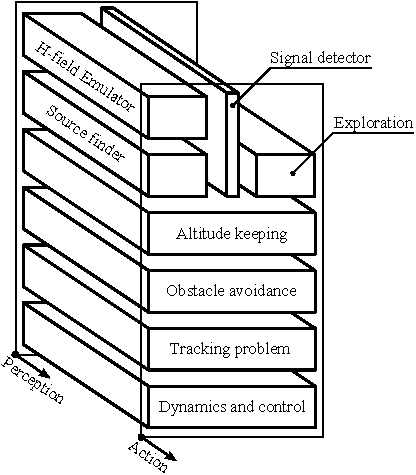
\includegraphics[scale=0.9]{ch3/img/PA_map_general.pdf}

	\begin{tikzpicture}[>=latex']
		\drawplanexy{-0.3}{-0.3}{-0.3}{6.7}{10}{dashed}{perception}
		\node [at=(perception_D),xshift=30,yshift=-10] {\textbf{Perception}};
		\drawcube{0}{0}{5}{6.4}{1}{white}{dinamica}{Dynamics and control}{};
		\drawcube{0}{1.2}{5}{6.4}{1}{white}{tracking}{Tracking Problem}{};
		
		\drawcube{0}{2.4}{5}{6.4}{1}{white}{ostacoli}{Obstacle Avoidance}{};
		\drawcube{0}{3.6}{5}{6.4}{1}{white}{altitude}{Altitude Keeping}{};
		
		\drawcube{0}{4.8}{5}{3}{1.5}{white}{source}{Source searching}{text width=2cm,align=center};
		\drawcube{0}{6.5}{5}{3}{1.5}{white}{emulatore}{Emulation}{text width=2cm,align=center};

		\drawplanezy{3.2}{4.8}{5}{4.5}{radar_det}{fill=white,opacity=0.90}{Radar detect}{rotate=45,xslant=1};

		\drawcube{3.4}{4.8}{5}{3}{3.2}{white}{alpha}{Exploration routines}{text width=2cm,align=center};
		\drawplanexy{-0.3}{-0.3}{5.3}{6.7}{10}{dashed}{action}
		\node [at=(action_D),xshift=20,yshift=-10] {\textbf{Action}};

		\draw [->,line width=1.5] (action_D) -- ++(0,0,2);
		\draw [->,line width=1.5] (perception_D) -- ++(0,0,2);

		\coordinate [at=(radar_det_D), yshift=-20] (arrows_point);
		\draw [->,dashed]  (arrows_point) -- ++(1.5,0,0); 
		\draw [->,dashed]  (arrows_point) -- ++(-1.5,0,0); 
	\end{tikzpicture}
	\forcerectofloat
	\caption{General Perception--Action map for our drone}
	\label{fig:genPAmap}
\end{figure}
\FloatBarrier
\section{Hexa--copter model}

The drone could be modeled with dynamical equations. The derivation of those equation will be performed from force analysis and control scheme is derived. A \texttt{C} version of the model, to be used in simulations is presented.

\subsection{Motion equations}
The system is governed by Euler--Newton equations, simplified with the imposition of the center of motion for Euler equations in center of mass of the drone. With character $g$ we refer to global coordinate system, while with $b$ we identify the coordinate system, that is attached to body and has origin in CoM:
\begin{equation}
\left\{
\begin{array}{rcl}
\totforcehexa_g & = & \massadrone \ddot{\hexastate}_g \\
\tottorquehexa_g & = & \dot{\mathbf{K}}_g + \dot{\hexastate}_g \times \mathbf{Q}_g%
\end{array}
\right.  \rightarrow  \left\{
\begin{array}{rcl}
\totforcehexa_b & = & m \mathbf{a}_b \\
\tottorquehexa_b & = & \dot{\mathbf{K}}_b%
\end{array}
\right.
\end{equation}
\myparagraph{External force and torque analysis}
There are several force that act on the body of the drone:
\begin{equation}
\totforcehexa_b = \sum\limits_{\mathrm{external}} F_b
\end{equation}

\textbf{Weight}:
\begin{equation}
\mathbf{P}_g = \vettore{0 \\ 0 \\ - m g}
\end{equation}

\textbf{Motor thrust}:
\begin{equation}
\mathbf{L}_b = \sum\limits_{i=1}^6 \vettore{0 \\ 0 \\ -L_{b,i}}
\end{equation}

\textbf{Total force}:
\begin{equation}
\totforcehexa_b = \vettore{\sin(\theta) \\ -\sin(\phi)\cos(\theta) \\ - \cos(\phi)\cos(\theta)} m g + \vettore{ 0 \\ 0 \\ - \sum\limits_{i=1}^6 L_{b,i}}
\end{equation}

For what concerns total external torque applied to the system:
\begin{equation}
\tottorquehexa_{b,\mathbf{0}} = \sum\limits_{\mathrm{external}} M_b + \sum\limits_{\mathrm{external}} (\mathbf{p}_b - \mathbf{0}) \times \totforcehexa_b
\end{equation}

\textbf{Thrust torque}, with $l$ distance between center of propeller and CoM
\begin{equation}
\mathbf{M}_b = \sum\limits_{i=0}^5 \vettore{ l \cos(i \pi/3) \\ l \sin(i \pi /3) \\ 0 } \times \mathbf{L}_{b,i}
\end{equation}

\textbf{Drag torque}, with $\beta$ the proportional factor between thrust and drag torque
\begin{equation}
\mathbf{D}_b = \sum\limits_{i=1}^6 \vettore{ 0 \\ 0 \\ \beta L_{b,i}}
\end{equation}

In general, the total torque is:
\begin{equation}
\tottorquehexa_{b,0} = \left[ \begin{array}{c}
-\dfrac{\sqrt{3}}{2} l \left( L_2 +L_3 - L_5 - L_6 \right) \\
\dfrac{1}{2} l \left( 2 L_1 + L_2 -L_3 - 2 L_4 - L_5 + L_6 \right) \\ 
\beta \left( L_1 - L_2 + L_3 - L_4 + L_5 - L_6 \right)
\end{array}
\right]
\end{equation}

\myparagraph{Inertial analysis}
We could define speed vector in body system of coordinates:
\begin{equation}
\vettore{\dot{x} \\ \dot{y} \\ \dot{z}} = \rotmat \vettore{u\\v\\w}
\end{equation}
\marginnote{The rotational matrix form body to ground is obtained through a sequence of elementary rotations:
${\mathcal{R} = \mathcal{R}_z(\psi)\;\mathcal{R}_y(\theta)\;\mathcal{R}_x(\phi)}$}.  that allows us to define the accelerations vector in the form:
\begin{equation}
\mathbf{a}_b = \dot{\mathbf{v}}_b + \boldsymbol{\omega}_b \times \mathbf{v}_b
\end{equation}
The relation that connects angular ratios in body coordinates and ground coordinates are derived from the so called \emph{Gimball's relations}\sidenote{Just a clarification on the notation used. Square parentheses $[\cdot]$ identifies vector element that belongs to the same basis, while vectorial elements in curly brackets $\{\cdot\}$ do not share the same basis}:
\begin{equation}
\boldsymbol{\omega}_b = \mathcal{R}_x (\phi) \dot{\phi} \vers{e}''_x + \mathcal{R}_x(\phi) \mathcal{R}_y(\theta) \dot{\theta} \vers{e}'_y + \mathcal{R}_x(\phi) \mathcal{R}_y(\theta) \mathcal{R}_z(\psi) \dot{\psi} \vers{e}_z
\end{equation}
that is simplified in the matrix form:
\begin{equation*}
\left[ \begin{array}{c} p \\ q \\ r \end{array} \right] = \left[ \begin{array}{ccc}
 1 & 0 & -\sin(\theta) \\
 0 & \cos(\phi) & \sin(\phi)\cos(\theta) \\
 0 & -\sin(\phi) & \cos(\phi)\cos(\theta)
 \end{array} \right] \left\{ \begin{array}{c} \dot{\phi} \\ \dot{\theta} \\ \dot{\psi} \end{array} \right\}
\end{equation*}
that through inversion gives:
\begin{equation}
\left\{ \begin{array}{c} \dot{\phi} \\ \dot{\theta} \\ \dot{\psi} \end{array} \right\} = 
\left[ \begin{array}{ccc}
 1 & \dfrac{\sin(\phi) \sin(\theta)}{\cos(\theta)} &  \dfrac{\cos(\phi) \sin(\theta)}{\cos(\theta)}\\
 0 & \cos(\phi) & -\sin(\phi) \\
 0 & \dfrac{\sin(\phi)}{\cos(\theta)} & \dfrac{\cos(\phi)}{\cos(\theta)} 
 \end{array} \right]
\left[ \begin{array}{c} p \\ q \\ r \end{array} \right]
\end{equation}
For what concerns angular inertia in body reference frame:
\begin{equation}
\begin{array}{rcl}
\dot{\mathbf{K}}_b &=& \matriceinerzia \dot{\boldsymbol{\omega}}_b + \boldsymbol{\omega}_b \times \matriceinerzia \boldsymbol{\omega}_b \\
&=& \left[ \begin{array}{c} I_x \dot{p} \\ I_y \dot{q} \\ I_z \dot{r} \end{array} \right] + \left[ \begin{array}{c} (I_z-I_y) q r \\ (I_x-I_z) p r \\ (I_y-I_x) p q \end{array} \right]
\end{array}
\end{equation}

\myparagraph{Newton--Euler equations}
Defined state vectors and control vectors:
\arraymath{%
\hexastate & = & \left[ x,y,z,u,v,w,\phi,\theta,\psi,p,q,r \right]^T \\
\hexacontrol & = & \left[ L_1, L_2, L_3, L_4, L_5, L_6 \right]^T%
}
we get the following Newton--Euler equations that describes dynamical behavior of the drone:
\begin{margintable}
	\renewcommand{\arraystretch}{1.2}
	\begin{center}
	\begin{tabular}{p{0.5cm} p{2cm} p{1.5cm}}
	\hline \textbf{Sym.} & \textbf{Description} & \textbf{Value} \\ \hline
	$g$     & Gravity        & $9.81 $ \si{\kilo\gram\per\square\second} \\
	$m$     & Mass           & $2$     \si{\kilo\gram}\\
	$I_x$   & $x$ Inertia    & $0.008$ \si{\kilo\gram\square\meter}\\
	$I_y$   & $y$ Inertia    & $0.01$  \si{\kilo\gram\square\meter}\\
	$I_z$   & $z$ Inertia    & $0.05$  \si{\kilo\gram\square\meter}\\
	$\beta$ & Drag parameter & $0.2$   \si{\kilo\gram\square\meter}\\
	$l$     & Frame arm      & $0.3$   \si{\meter} \\ \hline
	\renewcommand{\arraystretch}{1.75}
	\end{tabular}
	\end{center}
	\caption{Mechanicals parameters of the simulated model}
\end{margintable}
\begin{equation}
\left\{\begin{array}{rcl}
\dot{x} &=&\cos ( \psi) \cos ( \theta) u +\sin ( \psi) \cos ( \theta) v -\sin ( \theta) w \\
\dot{y} &=& \cos ( \psi ) u \sin ( \theta ) \sin ( \phi) +\sin( \psi) v \sin ( \theta) \sin ( \phi ) + \\ & &  +\cos ( \psi) v  \cos ( \phi) +\cos ( \theta) \sin ( \phi ) w -u \sin ( \psi) \cos ( \phi) \\
\dot{z} & = &\cos ( \psi) u \sin ( \theta ) \cos ( \phi) +\sin( \psi) v \sin ( \theta) \cos ( \phi ) + \\ & & -\cos ( \psi) v  \sin ( \phi) +\cos (\theta) \cos ( \phi ) w +u \sin ( \psi) \sin ( \phi) \\
\dot{u} & = & - q\;w + r\;v + g \sin(\theta) \\
\dot{v} & = & - r\;u + p\;w - g \sin(\phi) \cos(\theta) \\
\dot{w} & = & - p\;v + q\;u - g \cos(\theta) \cos(\phi) + \\ & &-\dfrac{1}{m} \left(L_1 + L_2 + L_3 + L_4 + L_5 + L_6 \right) \\

\dot{\phi} & = & p + \dfrac{\sin(\phi) \sin(\theta)}{\cos(\theta)}\;q + \dfrac{\cos(\phi) \sin(\theta)}{\cos(\theta)}\;r \\
\dot{\theta} & = & \cos(\phi)\;q - \sin(\phi)\;r \\
\dot{\psi} & = & \dfrac{\sin(\phi)}{\cos(\theta)}\;q + \dfrac{\cos(\phi)}{\cos(\theta)}\;r \\
\dot{p} & = & -\dfrac{I_z-I_y}{I_x} q\;r -\dfrac{\sqrt{3}}{2}\;\dfrac{l}{I_x}\;\left( L_2 +L_3 - L_5 - L_6 \right) \\
\dot{q} & = & -\dfrac{I_x-I_z}{I_y} p\;r + \dfrac{1}{2}\;\dfrac{l}{I_y}\;\left( 2 L_1 + L_2 -L_3 - 2 L_4 - L_5 + L_6 \right) \\
\dot{r} & = & -\dfrac{I_y-I_x}{I_z} p\;q + \dfrac{\beta}{I_z}\;\left( L_1 - L_2 + L_3 - L_4 + L_5 - L_6 \right)
\end{array}\right.
\end{equation}

\subsection{Linearization and LQR control}
\myparagraph{Linearization}
We now linearize the system feedback to get a control that stabilizes our drone:
\begin{equation}
\hexacontrol_0 \; : \; \mathbf{0}=f(\hexastate_0, \hexacontrol_0)
\end{equation}
that will be solved for hovering state, that is one of the most important flight routine. In a drone, hovering is not dependent with respect to vertical orientation along $\vers{z}$ axis:
\[
\hexastate = \left[ x_0, y_0, z_0,0,0,0,0,0,\psi_0,0,0,0 \right]^T
\]
One solution for this state is the control vector composed by thrust forces:
\[
L_1 = L_2 = L_3 = L_4 = L_5 = L_6 = \dfrac{mg}{6}
\]
and the linearized system is in the form:
\begin{equation}
\dot{\hexastate} = \underset{A}{\underbrace{\dfrac{\partial f(\hexastate,\hexacontrol)}{\partial \hexastate} \Big\rfloor_{\hexastate_0,\hexacontrol_0}}} \hexastate + \underset{B}{\underbrace{\dfrac{\partial f(\hexastate,\hexacontrol)}{\partial \hexacontrol} \Big\rfloor_{\hexastate_0,\hexacontrol_0}}} \hexacontrol
\end{equation}
and it is possible to obtain a representation of a linear model using a computer algebra system:
\renewcommand{\arraystretch}{1}
\begin{equation}
A = \left[ \begin{array}{cccccccccccc} 0&0&0&\cos \left( \psi_{{0}}
 \right) &\sin \left( \psi_{{0}} \right) &0&0&0&0&0&0&0
\\  0&0&0&-\sin \left( \psi_{{0}} \right) &\cos
 \left( \psi_{{0}} \right) &0&0&0&0&0&0&0\\  0&0&0&0&0
&1&0&0&0&0&0&0\\  0&0&0&0&0&0&0&g&0&0&0&0
\\  0&0&0&0&0&0&-g&0&0&0&0&0\\  0&0&0
&0&0&0&0&0&0&0&0&0\\  0&0&0&0&0&0&0&0&0&1&0&0
\\  0&0&0&0&0&0&0&0&0&0&1&0\\  0&0&0
&0&0&0&0&0&0&0&0&1\\  0&0&0&0&0&0&0&0&0&0&0&0
\\  0&0&0&0&0&0&0&0&0&0&0&0\\  0&0&0
&0&0&0&0&0&0&0&0&0\end{array} \right]
\end{equation}
\begin{equation}
B = \left[ \begin {array}{cccccc} 0&0&0&0&0&0\\  0&0&0&0
&0&0\\  0&0&0&0&0&0\\  0&0&0&0&0&0
\\  0&0&0&0&0&0\\   -\dfrac{1}{m}& -\dfrac{1}{m}& -\dfrac{1}{m}& -\dfrac{1}{m}& -\dfrac{1}{m}& -\dfrac{1}{m}\\  0&0&0&0
&0&0\\  0&0&0&0&0&0\\  0&0&0&0&0&0
\\  0&-\dfrac{\sqrt{3}}{2}\dfrac{l}{I_x}&-\dfrac{\sqrt{3}}{2}\dfrac{l}{I_x}&0&
\dfrac{\sqrt{3}}{2}\dfrac{l}{I_x}&\dfrac{\sqrt{3}}{2}\dfrac{l}{I_x}\\  \dfrac{l}{I_y}&\dfrac{1}{2}\dfrac{l}{I_y}&-\dfrac{1}{2}\dfrac{l}{I_y}&-\dfrac{l}{I_y}&-\dfrac{1}{2}\dfrac{l}{I_y}&\dfrac{1}{2}\dfrac{l}{I_y}
\\  \dfrac{\beta}{I_z}&-\dfrac{\beta}{I_z}&\dfrac{\beta}{I_z}&-\dfrac{\beta}{I_z}&\dfrac{\beta}{I_z}&-\dfrac{\beta}{I_z} \end {array} \right]
\end{equation}
\renewcommand{\arraystretch}{1.75}

\myparagraph{LQR on complete state}
From our linear system:
\begin{equation}
\dot{\hexastate} = A \hexastate + B \hexacontrol
\end{equation}
given the quadratic control cost function, with infinite horizon:
\[
J = \int\limits_{0}^{\infty} \hexastate^T Q \hexastate + \hexacontrol^T R \hexacontrol\, dt
\]
with $Q$ and $R$ positive defined.The optimum control that minimize this functional is: 
\begin{equation}
\hexacontrol^* = - R^{-1} B^T P \hexastate
\end{equation}
where $P$ is the solution of \emph{Riccati's equation}:
\[
A^T P + PA - P B R^{-1} B^T P + Q = 0
\]
the solution of this equation is obtain through numerical tools such as Matlab's \texttt{lqr} algorithm. Unfortunately it is impossible to derive analytical solution, given a wise chose of $Q$ and $R$ matrix. Usually, and also in this case, it is a good idea to follow the Bryson estimation (diagonal matrix, with higher weight to $Q$ matrix, or \emph{cheap control}):
\[
\begin{array}{rcl}
Q & = & \mathrm{eye}\left( q_i \; : \; i = 1..12 \right) \\
R & = & \rho \mathbb{I}_{6\times 6}
\end{array}
\]
whit the additional constraint to keep observability and controllability on couples:
\begin{margintable}
\renewcommand{\arraystretch}{1}
	\begin{centering}
	\begin{tabular}{p{1.5cm} p{1.5cm}}
		\hline
		\textbf{Parameter} & \textbf{Value} \\
		\hline
		$q_1$    & $10$ \\
		$q_2$    & $10$ \\
		$q_3$    & $2.5$ \\
		$q_4$    & $0.01$ \\
		$q_5$    & $0.01$ \\
		$q_6$    & $0.01$ \\
		$q_7$    & $20$ \\
		$q_8$    & $20$ \\
		$q_9$    & $10$ \\
		$q_{10}$ & $15$ \\
		$q_{11}$ & $15$ \\
		$q_{12}$ & $5$ \\
		$\rho$   & $1$ \\ \hline
	\end{tabular}
	\end{centering}
	\caption{Functional weights}
\renewcommand{\arraystretch}{1.75}	
\end{margintable}
\[
\begin{array}{rcl}
\mathcal{O}\braces{A,\sqrt{Q}} & = & \mathrm{rank}\braces{ \sqrt{Q}^T\;A^T\sqrt{Q}^T\;\dots\;\braces{A^T}^{\dim(\hexastate)-1}\sqrt{Q}^T} = 12 \\
\mathcal{C}\braces{A,B} & = & \mathrm{rank}\braces{ B\;A B\;\dots\;\braces{A}^{\dim(\hexastate)-1}B} = 6
\end{array}
\]

\myparagraph{Solving tracking problem}
It is really simple to solve a tracking problem starting from an LQR, that tries always to reach a zero. Simply insert an offset in position, and the system will try to reduce the error until it reach zero. Here we have a figure that explains the complete control, and some simulation test for random initial conditions that tries to reach a specific position in space.
\TODO{inserire immagine del controllo}



\section{Obstacle avoidance}
\begin{marginfigure}
	\centering
	%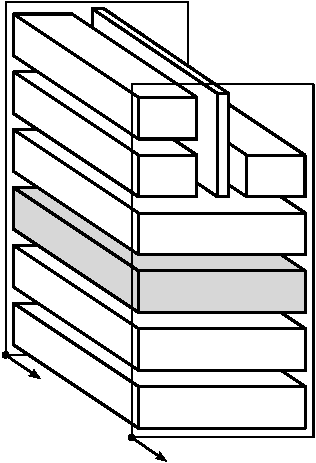
\includegraphics[scale=0.5]{ch3/img/PA_map_obstacle.pdf}
	\begin{tikzpicture}[>=latex',scale=0.4]
	\drawplanexy{-0.3}{-0.3}{-0.3}{6.7}{10}{dashed}{perception}
	
	\drawcube{0}{0}{5}{6.4}{1}{white}{dinamica}{}{};
	\drawcube{0}{1.2}{5}{6.4}{1}{white}{tracking}{}{};
	
	\drawcube{0}{2.4}{5}{6.4}{1}{gray!40}{ostacoli}{}{};
	\drawcube{0}{3.6}{5}{6.4}{1}{white}{altitude}{}{};
	
	\drawcube{0}{4.8}{5}{3}{1.5}{white}{source}{}{};
	\drawcube{0}{6.5}{5}{3}{1.5}{white}{emulatore}{}{};

	\drawplanezy{3.2}{4.8}{5}{4.5}{radar_det}{fill=white,opacity=0.90}{}{};

	\drawcube{3.4}{4.8}{5}{3}{3.2}{white}{alpha}{}{};
	\drawplanexy{-0.3}{-0.3}{5.3}{6.7}{10}{dashed}{action}
	

	\draw [->,line width=1.5] (action_D) -- ++(0,0,2);
	\draw [->,line width=1.5] (perception_D) -- ++(0,0,2);

	\coordinate [at=(radar_det_D), yshift=-5] (arrows_point);
	\draw [->,dashed]  (arrows_point) -- ++(1.5,0,0); 
	\draw [->,dashed]  (arrows_point) -- ++(-1.5,0,0); 
\end{tikzpicture}
\end{marginfigure}
An avalanche has an huge amount of kinetic energy, enough to destroy most of the artificial building and move objects with a big cross--section that are on its traveling path. Thus, the objects that avalanche drone has to avoid are mainly pillars, trees or mounds of snow.

Taken into account this consideration about the surroundings in which the drone will try to find a buried person, it is useless to define an internal map of obstacle and elaborate the optimal trajectory to an ending point because, in fact, for the most of the time the drone will explore without having such a knowledge of the ending point.

This simplification gather different advantage to the final algorithm:
\begin{itemize}
\item we do not need the extremely high computational power needed to maintain such environment projection into agent mind space
\item the obstacle avoidance imposes minor constraints on the upper layer of the searching algorithm, with respect to convoluted algorithm
\item the simplification brings to a more reliable routine, because of its deterministic nature, with respect to a Bayesian based map
\item this algorithm fits technical specification imposed by used hardware
\end{itemize}
while the main drawbacks are
\begin{itemize}
\item we are flying on a non optimal path
\item it is based on a simplification, and real life is always harder than what we aspect
\end{itemize}

Diving into deep, the definition is based upon the presence of one range finder for each arm of the drone. As range finder it is possible to use ultrasonic range finders, that are device that do not have problems on lens like laser ones. An ultrasonic range finder has a characteristic lobe, similar to an antenna directivity lobe, with a peak at almost \num{6}\si{\meter}. 

The algorithm tries to identify a run away speed, given the distance from the obstacle received from each sensor (${d_i\,:\,i=1..6}$):

\begin{equation}
\mathbf{v} = \rotmat \sum\limits_{i=1}^{6}v(d_i)\vettore{\cos\braces{(i-1)\dfrac{\pi}{3}} \\ -\sin\braces{(i-1)\dfrac{\pi}{3}} \\0}
\end{equation}

where ${v(d_i)}$ is a function that defines the velocity magnitude on the direction of the range finder. The first magnitude used was:
\begin{equation}
v(d_i) = - \dfrac{1}{d_i}
\end{equation}
that has some discontinuity problems, so the next function implemented is a sigmoid function:
\begin{equation}
v(d_i) = p_3 \braces{\dfrac{1}{1+e^{4 \braces{\frac{p_1}{2}-d_i}\frac{p_2}{p_3}}}-1}
\end{equation}
\begin{marginfigure}
	\centering
	%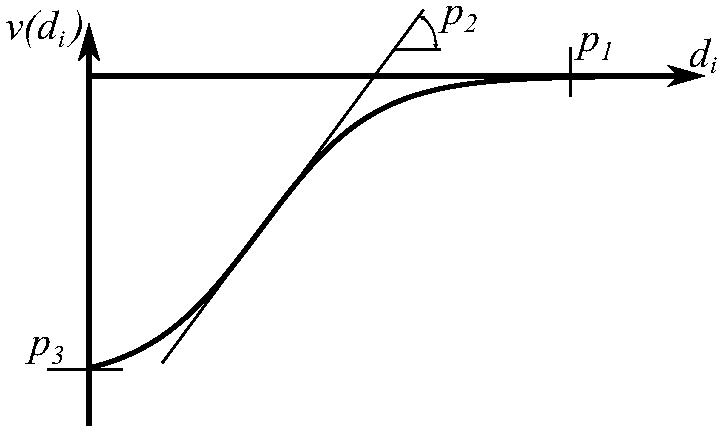
\includegraphics[scale=0.4]{ch3/img/speed_profile.pdf}
	\pgfmathdeclarefunction{speed}{3}{%
		\pgfmathparse{#3 * ( (1)/(1+exp(4*((#1/2)-x)*#2/#3)) - 1 )}%
	}
	\begin{tikzpicture}[>=latex]
		\begin{axis}[
			domain=0:11.5, samples=100,
			enlargelimits=false,
			xmin=0, xmax=12, ymin=-6, ymax=1,
			height=6cm, width=6cm,
			axis lines=middle,
			xlabel=\scriptsize{$d_i$}, ylabel=\scriptsize{$v(d_i)$},
			every axis y label/.style={at=(current axis.above origin),anchor=south },
			every axis x label/.style={at=(current axis.right of origin),anchor=west},
			xtick=\empty, ytick=\empty,
			extra y ticks={-4.7}, extra y tick labels={$p_3$},
			extra x ticks={10}, extra x tick labels={$p_1$}
		]
			\addplot[black,line width=1.5]{speed(7,1,5)};
		\end{axis}
		
		\draw (0.75,1.3) -- ++(240:1) -- ++(60:5) -- ++(240:0.75) -- ++(0.75,0) --++(-0.15,0) coordinate(arco);
		\draw[<->] (arco) arc(0:60:0.6) node [xshift=15] {$p_2$};	
	\end{tikzpicture}
	\caption{Velocity profile}
\end{marginfigure}
from which we obtain a continuous function where the parameters:
\begin{itemize}
\item $p_1$: it is the maximum range, at which considered velocity is zero
\item $p_2$: defines the slope of the curve at ${d_i = p_1/2}$
\item $p_3$: defines the maximum velocity, or the value of the curve for ${d_i = 0}$
\end{itemize}

In figure \ref{fig:obstavoidexample} an example of how the algorithm works is shown. Obviously, signal coming from the algorithm get some sort of filtration to eliminate various source of noise.
\begin{figure}[h]
	\centering
	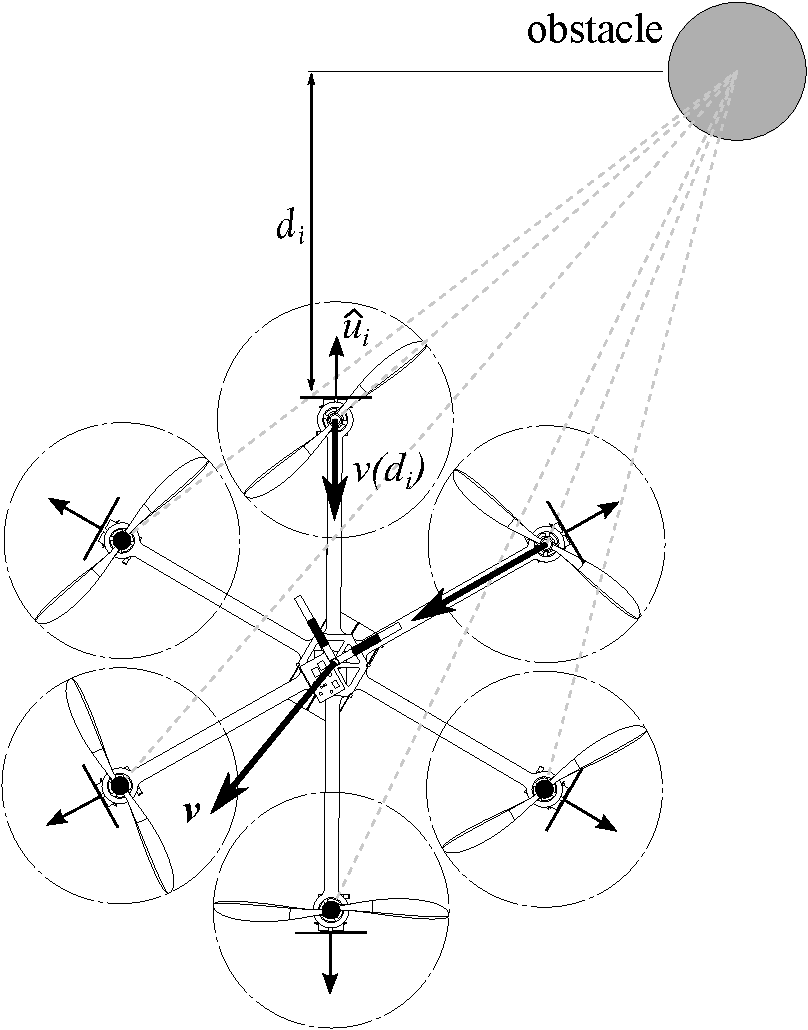
\includegraphics[scale=0.45]{ch3/img/obstavoid_dist.pdf}
	\caption{Example of obstacle avoid algorithm behavior}
	\label{fig:obstavoidexample}
	\forceversofloat
\end{figure}

\myparagraph{Model of range finder}
From the simulation point of view the effects of an obstacle are obtained through a model of the characteristic lobe of each range finder. 
\begin{figure}[h]
	\centering
	%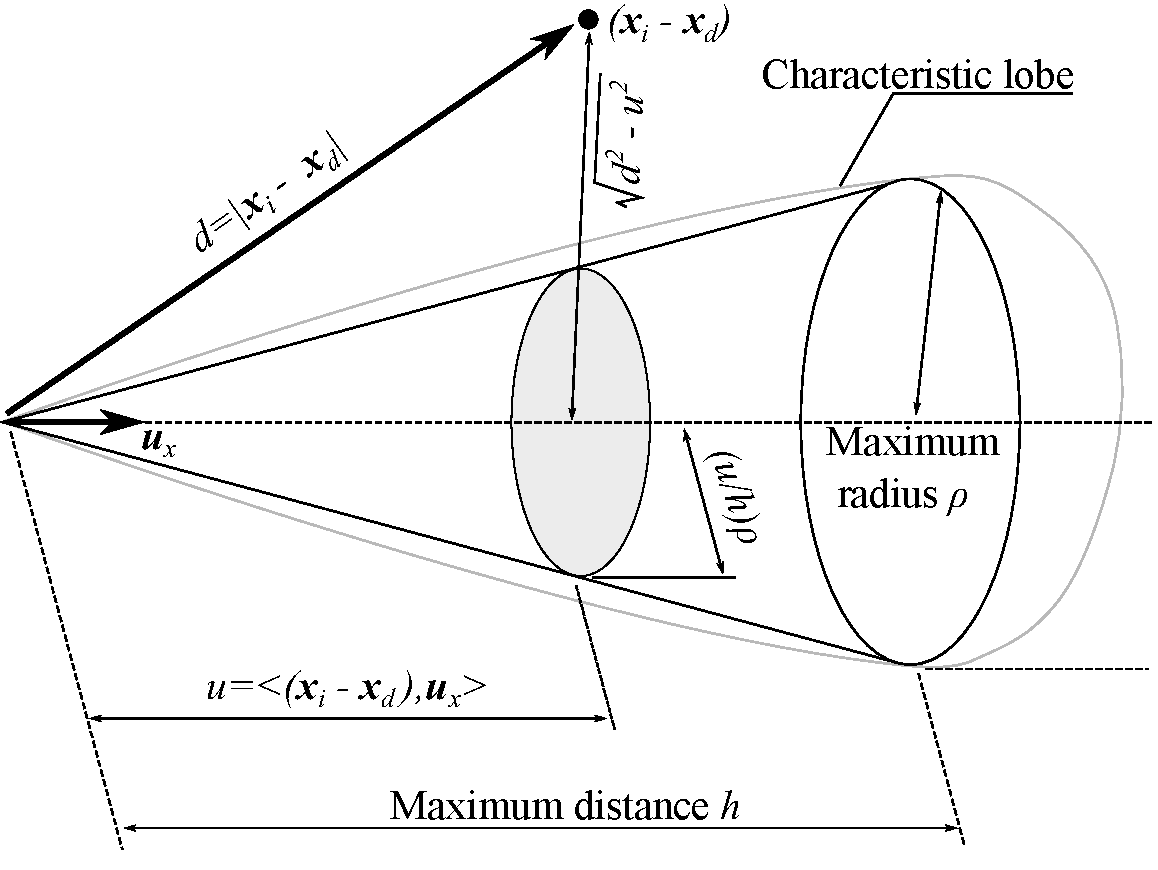
\includegraphics[scale=0.45]{ch3/img/lobe_dimensions.pdf}
	\begin{tikzpicture}[>=latex']
		\draw[dashed,gray] (0,0) .. controls (6cm,3cm) ..  (8.5cm,3.5cm) to[bend left,out=45] (11cm,0cm) to [bend left,in=125] (8.5cm,-3.5cm) .. controls (6cm,-3cm) .. cycle;
	   \draw [fill=gray!40,opacity=40](5cm,0cm) ellipse (0.75cm and 2.05cm);
		\draw (8.5cm,0cm) ellipse (1.25cm and 3.5cm);
		\draw (8.2cm,-3.4cm) -- (0,0) -- (8.2cm,3.4cm);
		\draw[dashed] (0,0) -- (9cm,0);

		\node [circle,inner sep=1pt,fill=black] at (5cm,4cm) {};
		\draw [<->] (5cm,0cm) -- node[pos=0.9,right]{$\sqrt{d_i^2-u^2}$} (5cm,3.9cm);
		\draw [->,line width=1.5] (0cm,0cm) -- (2.5cm,0cm);
		\draw [->,line width=1.5] (0cm,0cm) -- node[above,rotate=38.53]{$d_i = | \mathbf{x}_i^{\Psi} - \mathbf{x}_d|$} (4.9cm,3.9cm);
		\draw [->] (5cm,0cm) -- ++(-70:1.4) node[anchor=west,xshift=3,yshift=-3] {$\dfrac{\rho}{h}u$};
		\node at(4cm,4.3cm) {$(\mathbf{x}_i^{\Psi} - \mathbf{x}_d)$};
		\node at(2.5cm,-0.35cm) {$\hat{\mathbf{u}}_{i}$};

		\draw [->] (8.5cm,0cm) -- ++(-70:2.5) node[anchor=west,xshift=3,yshift=-3] {$\rho$ (maximum radius)};

		\draw (0cm,-0.1cm) -- (0cm,-5cm);
		\draw (4.9cm,-2.2cm) -- (4.9cm,-4cm);
		\draw (8.5cm,-0.1cm) -- (8.5cm,-5cm);
		\draw [<->](0cm,-3.9cm) -- node[pos=0.5,above]{$u=(\mathbf{x}_i^{\Psi} - \mathbf{x}_d) \cdot \hat{\mathbf{u}}_i$} (4.9cm,-3.9cm);
		\draw [<->](0cm,-4.9cm) -- node[pos=0.5,above]{$h$ (maximum range)} (8.5cm,-4.9cm);
		\draw [<-] (9cm,3.5cm) -- ++(45:0.5cm) -- node[pos=0.5,above]{Characteristic lobe} ++(3cm,0); 
	\end{tikzpicture}
	\caption{Range finder algorithm}
	\forcerectofloat
\end{figure}
The obstacles are implemented as sets of points, paradigm that brings a little advantage from the simulation point of view of inserting some noise due to the discontinuities between points, similar to real range finder noise, due to analog to digital conversion.
\begin{equation}
\Psi = \left[ \mathbf{x}_i \,:\,i=1..M  \right]
\end{equation}

For our system we suppose to know exactly the position $\hexastate_d$ and orientation $\rotmat$ of the drone\sidenote{For the obstacle avoidance algorithm only attitude must be know, to project the velocity in ground reference frame}. We define observation versors as follows:
\begin{equation}
\label{eq:versorirangefind}
\left\{ \vers{u}_i \,:\, i=1..6 \right\} \rightarrow \left\{ \vettore{\cos\braces{(i-1)\dfrac{\pi}{3}} \\ -\sin\braces{(i-1)\dfrac{\pi}{3}} \\0} \,:\, i=1..6 \right\}
\end{equation}
The characteristic of the range finder is described with the use of a cone. Distance is evaluated using time of flight of an ultrasonic signal emitted by the oscillator. Mathematically it is possible to define the lobe with a cone in the space, that has axis parallel to the versors defined in \ref{eq:versorirangefind}, and vertex coincident with receiving system. The solid that approximates the characteristic lobe is defined by:
\begin{equation}
\begin{array}{rcl}
x &=& \dfrac{u}{h} \rho \cos(\theta) \\
y &=& \dfrac{u}{h} \rho \sin(\theta) \\
z &=& u
\end{array}
\end{equation}
where the parameters:
\begin{itemize}
\item $h$: receiver maximum distance
\item $\rho$: receiver maximum lobe dimension
\end{itemize}

\begin{algorithm}[h]
\label{alg:rangefinder}
\caption{Range finder points}
\SetKw{KwAs}{as}
\KwData{$h,\,\rho$}
\ForEach{Obstacle \KwAs $\Psi$}{
	\tcc{Exec for each point of an obstacle}
	\For{$i=1$ \KwTo $M$}{ 
		${\mathbf{d}_i^{\Psi} \leftarrow \mathcal{R}^T(\phi,\theta,\psi) \braces{\mathbf{x}_{i,\mathrm{ground}}^{\Psi}-\mathbf{x}_d}}$\;
		\For{$j=0$ \KwTo 5}{
			${D_{i,j}^{\Psi} \leftarrow \mathbf{d}_i^{\Psi} \cdot \vers{u}(j\pi/3)}$\;
			\tcc{Check if the point is in cone, else distance is $\infty$}
			\eIf{$\braces{0\leq D_{i,j}^{\Psi} \leq h}$}{
				\If{$\braces{\mathbf{d}_i^{\Psi} \cdot \mathbf{d}_i^{\Psi} - {D_{i,j}^{\Psi}}^2 \geq \braces{\dfrac{\rho}{h} D_{i,j}^{\Psi}}^2 }$}{
					${D_{i,j}^{\Psi} \leftarrow \infty}$\;
				}
			}{
				${D_{i,j}^{\Psi} \leftarrow \infty}$ \;
			}
		}
	}
}
\tcc{Search minimum distance for each sensor}
$\mathbf{r} \leftarrow [r_j = \infty\,:\,j=0$ \KwTo $5]$\;
\For{$j=0$ \KwTo 5}{
	\ForEach{Obstacle \KwAs $\Psi$}{
		\For{$i=1$ \KwTo $M$}{
			\If{$r_j \geq D_{i,j}^{\Psi}$}{
				$r_j \leftarrow D_{i,j}^{\Psi}$ \;
			}
		}
	}
}
\Return{$\mathbf{r}$}
\end{algorithm}

Given a point ${\mathbf{x}_i \in \Psi}$, if it is inside the cone, the projection of the distance ${\mathbf{x}_d-\mathbf{x}_i}$ on the axis of the cone is the identified distance.

The algorithm describes how each sensor returns the minimum identified distance that is inside its cone. The distances are used to build the velocity vector that avoid the obstacle.

\FloatBarrier
\section{Altitude keeping}
\begin{marginfigure}
	\centering
	%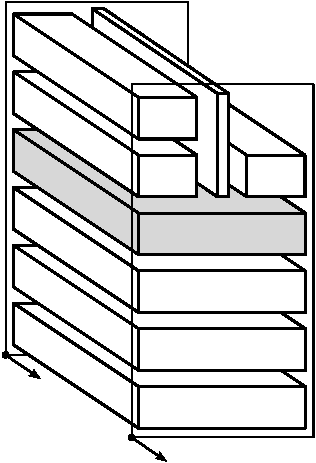
\includegraphics[scale=0.5]{ch3/img/PA_map_altitude.pdf}
	\begin{tikzpicture}[>=latex',scale=0.4]
	\drawplanexy{-0.3}{-0.3}{-0.3}{6.7}{10}{dashed}{perception}
	
	\drawcube{0}{0}{5}{6.4}{1}{white}{dinamica}{}{};
	\drawcube{0}{1.2}{5}{6.4}{1}{white}{tracking}{}{};
	
	\drawcube{0}{2.4}{5}{6.4}{1}{white}{ostacoli}{}{};
	\drawcube{0}{3.6}{5}{6.4}{1}{gray!40}{altitude}{}{};
	
	\drawcube{0}{4.8}{5}{3}{1.5}{white}{source}{}{};
	\drawcube{0}{6.5}{5}{3}{1.5}{white}{emulatore}{}{};

	\drawplanezy{3.2}{4.8}{5}{4.5}{radar_det}{fill=white,opacity=0.90}{}{};

	\drawcube{3.4}{4.8}{5}{3}{3.2}{white}{alpha}{}{};
	\drawplanexy{-0.3}{-0.3}{5.3}{6.7}{10}{dashed}{action}
	

	\draw [->,line width=1.5] (action_D) -- ++(0,0,2);
	\draw [->,line width=1.5] (perception_D) -- ++(0,0,2);

	\coordinate [at=(radar_det_D), yshift=-5] (arrows_point);
	\draw [->,dashed]  (arrows_point) -- ++(1.5,0,0); 
	\draw [->,dashed]  (arrows_point) -- ++(-1.5,0,0); 
\end{tikzpicture}
\end{marginfigure}
The last basic block that should be implemented is the altitude keeping, to maintain the distance of the drone to the soil high enough to avoid contact with rescuer and low enough to get a good signal strength. The sensors used are, again, ultrasonic range finder. With respect to the obstacle avoidance, that acts as a control on the lateral dynamic of the drone, that is quite slow, altitude keeping works on vertical dynamic that is really fast, and need a more reliable implementation, and require a statistical system to determine the distance even with a high irregular terrain.

This part was actually not implemented because of the need of more test about response of ultrasonic waves upon snow surface, to better understand the effects of density on perceived distance.

\subsection{Kalman Filter}
We assume that the dimension could be described with the use of normal distribution:
\begin{equation}
p(\hexastate) \det\braces{(2\pi)^{n}\Sigma_0}^{-1/2} e^{-\dfrac{1}{2}\braces{\hexastate - \boldsymbol{\mu}}^T \Sigma^{-1}\braces{\hexastate - \boldsymbol{\mu}}}
\end{equation}
with ${\boldsymbol{\mu}}$ the mean value for the distribution and ${\Sigma}$ covariance matrix of the distribution.

The Kalman filter include the knowledge of the covariance matrix into the state estimation procedure, and it is possible to proof that the final estimation will maintain a normal distribution if:
\begin{itemize}
\item distribution of initial state is normal
\item the state distribution is a linear function of the previous state and a white Gaussian noise
\item the measurement distribution  is a linear function of the state and a white Gaussian noise
\end{itemize}

\myparagraph{Initial state probability}
We make the really strong hypothesis to have an initial distribution in the normal form:
\begin{equation}
p(\hexastate_0) \det\braces{(2\pi)^{n}\Sigma_0}^{-1/2} e^{-\dfrac{1}{2}\braces{\hexastate_0 - \boldsymbol{\mu_0}}^T \Sigma_{0}^{-1}\braces{\hexastate_0 - \boldsymbol{\mu_0}}}
\end{equation}

\myparagraph{Prediction phase}
The distribution of the state derives from the distribution of the previous state, using the linear relation:
\begin{equation}
\hexastate_t = A_t \hexastate_{t-1} + B \hexacontrol_t + \statenoise
\end{equation}
where ${\mathbf{w}_t}$ is a realization of a distribution ${\mathcal{N}(\mathbf{0},R_t)}$ in which $R_t$ is the matrix that describes the covariance of the noise on the state.

The distribution is normal due to the relations:
\arraymath{
\bar{\boldsymbol{\mu}_{t}} &=& A_t \boldsymbol{\mu}_{t-1} + B_t \hexacontrol_{t} \\
\bar{\Sigma_{t}} &=& A_t \Sigma_{t-1} A_t^T + R_t \\
p(\hexastate_t \mid \hexastate_{t-1}, \hexacontrol_t) &=& \det((2\pi)^n R_t)^{-\frac{1}{2}} e^{\left( - \frac{1}{2} (\hexastate_t - \bar{\boldsymbol{\mu}_{t}})^T {R_t}^{-1} (\hexastate_t - \bar{\boldsymbol{\mu}_{t}}) \right)}
}

If the system has a non--linear function that describes the dynamic, it could be approximated with a first--order Taylor expansion:
\begin{equation}
\hexastate_t = g\braces{\hexastate_{t-1},\hexacontrol_t} + \statenoise
\end{equation}
\arraymath{
\mathrm{Taylor}_{1}\left(g(\hexastate_{t-1},\hexacontrol_t)\right)\Big\rfloor_{\bar{\boldsymbol{\mu}}_{t-1},\bar{\hexacontrol}_t} & = & g(\bar{\boldsymbol{\mu}}_{t-1},\bar{\hexacontrol}_t) + \\ & & \nabla_{\hexastate} g (\hexastate_{t-1},\hexacontrol_t)\Big\rfloor_{\bar{\boldsymbol{\mu}}_{t-1},\bar{\hexacontrol}_t}\left( {\hexastate}_{t-1} - \bar{\boldsymbol{\mu}}_{t-1} \right) \\
& = & g(\bar{\boldsymbol{\mu}}_{t-1},\bar{\hexacontrol}_t) + A_t\left( {\hexastate}_{t-1} - \bar{\boldsymbol{\mu}}_{t-1} \right)
}

\myparagraph{Estimation state}
The measurement distribution derives directly from the measurement model:
\begin{equation}
\mathbf{z}_t = C_t \hexastate_t + \measnoise
\end{equation}
where ${\mathbf{v}_t}$ is a realization of a distribution ${\mathcal{N}(\mathbf{0},Q_t)}$ in which $Q_t$ is the matrix that describes the covariance of the noise on the measurement.

The distribution maintains its normal behavior due to the relation:
\[p(\mathbf{z}_t\mid\hexastate_t) = \det((2\pi)^n Q_t)^{-\frac{1}{2}} e^{\left( -\frac{1}{2} (\mathbf{z}_t - C_t \hexastate_t)^T Q_t^{-1} (\mathbf{z}_t - C_t \hexastate_t) \right)}\]

If the measurement is modeled with the use of a non--linear function it is possible to use a Taylor expansion to approximate locally the measurement function:
\begin{equation}
\mathbf{z}_t = h(\hexastate_t) + \measnoise
\end{equation}
\arraymath{
\mathrm{Taylor}_{1}\left(h(\hexastate_{t})\right)\Big\rfloor_{\bar{\boldsymbol{\mu}}_{t}} & = & h(\bar{\boldsymbol{\mu}}_{t}) + \nabla_{\hexastate} h (\hexastate_{t})\Big\rfloor_{\bar{\boldsymbol{\mu}}_{t-1}}\left( {\hexastate}_{t} - \bar{\boldsymbol{\mu}}_{t} \right) \\
 & = & h(\bar{\boldsymbol{\mu}}_{t}) + C_t\left( {\hexastate}_{t} - \bar{\boldsymbol{\mu}}_{t} \right)
}

\myparagraph{Complete KF algorithm}
Now we are ready to define a complete Kalman Filter. The blue lines represent the step that should be performed in the case of non--linear models. Must be noticed, that in case of such non--linearities, it is impossible to demonstrate the fact that normal posterior distribution are maintained.
\begin{algorithm}[h]
\caption{(Extended) Kalman Filter}
\KwData{$\stateest_{t-1},\,\statecovest_{t-1},\,\hexacontrol_t,\,\measset_t$}
\tcc{Prediction phase}
\eIf{Model is linear}{
	${\statepred_t = A_t \stateest_{t-1} + B_t \hexacontrol_t}$ \;
	${\measpred_t = C_t \statepred_t}$ \;
}{
	${\color{blue} \statepred_t = g\braces{\stateest_{t-1},\hexacontrol_t}}$ \;
	${\color{blue} A_t = \nabla_{\hexastate}g\braces{\hexastate_{t-1},\hexacontrol_t} \Big\rfloor_{\statepred_{t-1},\hexacontrol_t}}$ \;
	${\color{blue} B_t = \nabla_{\hexastate}h\braces{\hexastate_{t-1}} \Big\rfloor_{\statepred_{t-1},\hexacontrol_t}}$ \;
	${\color{blue} \measpred_t = h(\statepred_t)}$ \;
}
${\statecovpred_t = A_t \statecovpred_{t-1} A_t + \statecovnoise}$ \;
\tcc{Evaluation of Kalman Gain}
${\kfgain = \statecovpred_t C_t^T \braces{ C_t \statecovpred_t C_t^T + \meascovnoise }^{-1}}$ \;
\tcc{Estimation phase}
${\stateest_t = \statepred_t + \kfgain \braces{\measset_t - \measpred_t}}$ \;
${\statecovest_t = \braces{\mathbb{I} - \kfgain C_t} \statecovpred_t}$ \;
\Return{${\stateest_t,\,\statecovest_t}$}
\end{algorithm}
\FloatBarrier
\subsection{Application to altitude keeping}
\begin{figure}[h]
	\centering
	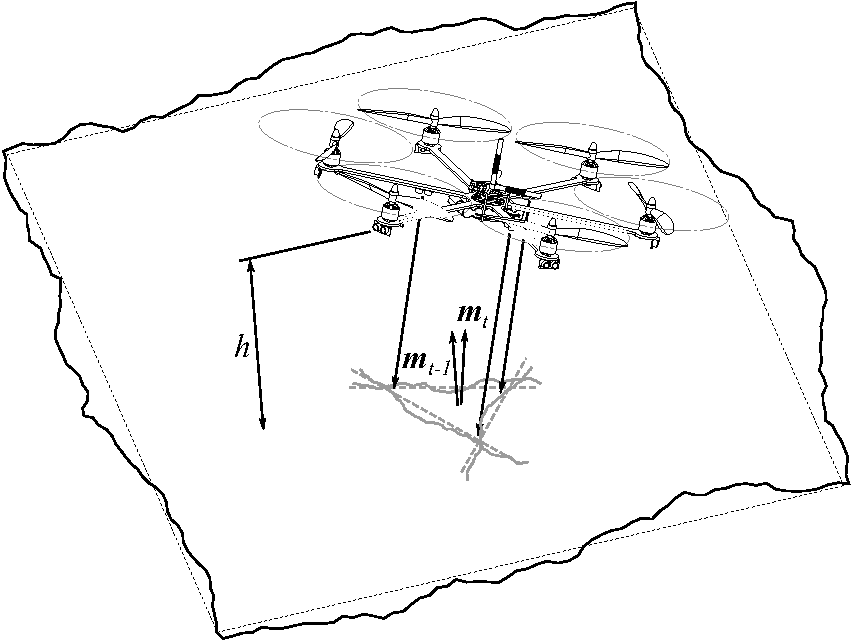
\includegraphics[scale=0.65]{ch3/img/altitude_keep.pdf}
	\caption{Altitude keeping problem}
	\forceversofloat
\end{figure}
\FloatBarrier
We can model the problem taking into account attitude dynamic and vertical dynamic of the VTOL, from which we know also the rotation matrix of the drone. The plane of the avalanche could be approximated through the orthogonal versor $\vers{m}$, projected in the drone reference frame. The problem, inserting $\vers{m}$ into the state vector, becomes equivalent to a \emph{SLAM}\sidenote[][-1cm]{\emph{SLAM}: Simultaneous Localization And Mapping} problem.

The state is:
\renewcommand{\arraystretch}{1}
\begin{equation}
\hexastate = \vettore{\hexastate \\ \vers{m}_b}
\end{equation}
\renewcommand{\arraystretch}{1.75}
and the covariance matrix of the state derives from covariance of the position system at which must be added a covarianc ematrix on the knowledge of ${\vers{m}_b = \rotmat^{T} \vers{m}}$. We could use three range finder directed to the ground, under the drone, that allow us to define three points on the surface. A model for the measurement function uses some simple algebraic definitions: given three points that belong to the plane, $\{A,\, B,\, C\}$, the normal is:
\begin{equation}
\vers{m} = \dfrac{(A-B)\times(B-C)}{\abs{(A-B)\times(B-C)}}
\end{equation}

Once normal is know, it could be used to implement a tracking control that maintains a certain distance on the normal vector. As already said, the performance of this algorithm depends directly from the estimation of the covariance matrix for measurement, and upon the sonar response due to variation of snow on the field.
%\FloatBarrier7
\section{The signal detection problem}
\begin{marginfigure}
	\centering
	%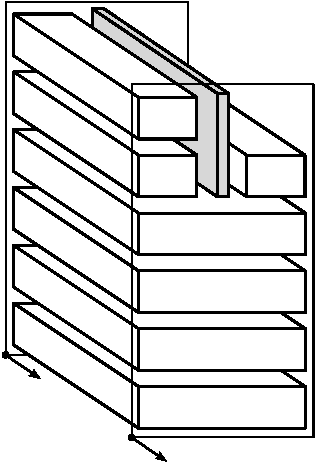
\includegraphics[scale=0.5]{ch3/img/PA_map_radar.pdf}
	\begin{tikzpicture}[>=latex',scale=0.4]
	\drawplanexy{-0.3}{-0.3}{-0.3}{6.7}{10}{dashed}{perception}
	
	\drawcube{0}{0}{5}{6.4}{1}{white}{dinamica}{}{};
	\drawcube{0}{1.2}{5}{6.4}{1}{white}{tracking}{}{};
	
	\drawcube{0}{2.4}{5}{6.4}{1}{white}{ostacoli}{}{};
	\drawcube{0}{3.6}{5}{6.4}{1}{white}{altitude}{}{};
	
	\drawcube{0}{4.8}{5}{3}{1.5}{white}{source}{}{};
	\drawcube{0}{6.5}{5}{3}{1.5}{white}{emulatore}{}{};

	\drawplanezy{3.2}{4.8}{5}{4.5}{radar_det}{fill=gray!40,opacity=0.90}{}{};

	\drawcube{3.4}{4.8}{5}{3}{3.2}{white}{alpha}{}{};
	\drawplanexy{-0.3}{-0.3}{5.3}{6.7}{10}{dashed}{action}
	

	\draw [->,line width=1.5] (action_D) -- ++(0,0,2);
	\draw [->,line width=1.5] (perception_D) -- ++(0,0,2);

	\coordinate [at=(radar_det_D), yshift=-5] (arrows_point);
	\draw [->,dashed]  (arrows_point) -- ++(1.5,0,0); 
	\draw [->,dashed]  (arrows_point) -- ++(-1.5,0,0); 
\end{tikzpicture}
\end{marginfigure}
We have two searching status for our agent. In one searching status, the VTOL tries to identify a signal, while in the second stage, once we have identified the presence of a signal, the drone has to find the transmission source point. The passage from a searching strategy to another is the\emph{supervised signal detection}.

\subsection{Supervised signal detection}
What we are trying to define is a strategy that is able to detect a target signal from a background noise. This is not new to signal theory, if we look at radar research work.
\begin{marginfigure}
	\centering
	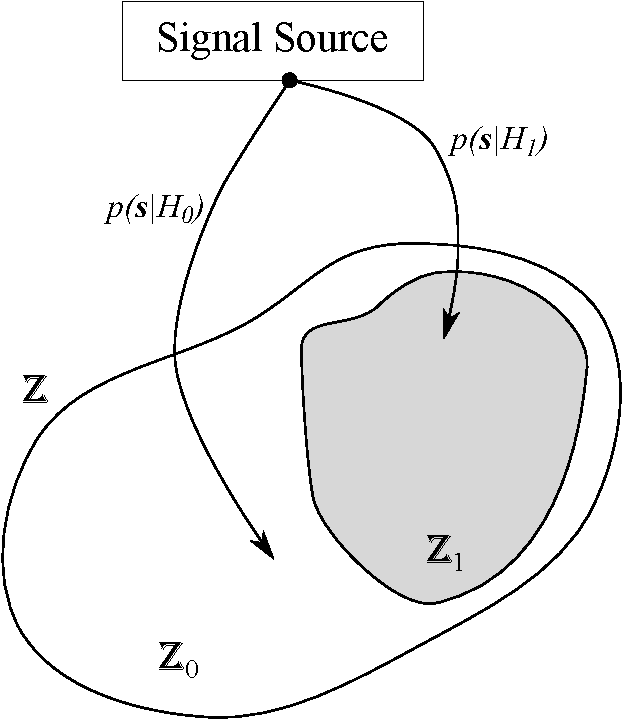
\includegraphics[scale=0.5]{ch3/img/signalsources.pdf}
	\caption{Decision spaces}
\end{marginfigure}
The detection theory is seen as a binary classification problem based upon two hypothesis:
\begin{itemize}
\item hypothesis $0$: absence of signal
\item hypothesis $1$: presence of signal
\end{itemize}
The choice is made upon a signal ${\signal = [s_1,\dots,s_n]}$ in which a certain number of feature identifies its belonging to a decision field or observation space $\decspace \in \mathbb{R}^n$. The observation space is defined by the union of two decision regions:
\[ \decspace \equiv \decspacezero \cup \decspaceone \]
Each decision space has a conditional \emph{PDF}, that is assumed to be known:
\arraymath{
	\decspacezero & \mapsto & p(\signal|\hypzero) \\
	\decspaceone & \mapsto & p(\signal|\hypone) \\
}

\subsection{Risk criterion}
The classification is based upon criteria, such as:
\begin{itemize}
\item Minimum Risk Criterion
\item Minimax Criterion
\item Neyman--Pearson Criterion
\end{itemize}
That represents the classification strategies.

\myparagraph{Minimum risk criterion}
This criterion is based upon the assumptions that posteriors probability ${P(\hypzero|\signal)}$ and ${P(\hypone|\signal)}$ are known, and also the cost matrix is known, where the matrix is defined in table \ref{tbl:cost_matrix}.
\begin{margintable}
	\renewcommand{\arraystretch}{1}
	\begin{centering} 
		\begin{tabular}{>{\centering} m{1.25cm} <{\centering} | >{\centering} m{1.25cm} <{\centering} >{\centering} m{1.25cm} <{\centering}}
		\hline										& \scriptsize{\textbf{Decide absent}\newline$D_0$} & \scriptsize{\textbf{Decide present}\newline$D_1$} \tabularnewline \hline
		\scriptsize{\textbf{Signal absent}\newline$\hypzero$}  	& \cellcolor{lgray}\scriptsize{Correct rejection:\newline$c_{0,0}$} & \cellcolor{dgray}\scriptsize{False alarm:\newline$c_{1,0}$}        \tabularnewline
		\scriptsize{\textbf{Signal present}\newline$\hypone$} 	& \cellcolor{dgray}\scriptsize{Miss:\newline$c_{0,1}$}              & \cellcolor{lgray}\scriptsize{Hit:\newline$c_{1,1}$}                \tabularnewline \hline
		\end{tabular}
	\end{centering} 
	\renewcommand{\arraystretch}{1.75}
	\caption{Costs matrix}
	\label{tbl:cost_matrix}
\end{margintable}
In practice we have: ${c_{0,1} > c_{1,1}}$ and ${c_{1,0} > c_{0,0}}$.

The main objective is to \emph{minimize the average cost incurred by erroneous decision}\TODO{citep libro pattrec}. This is done through a minimization of a risk function defined over observation space. This optimization allows us to define the decision regions $\decspacezero$ and $\decspaceone$ which are optimal in terminal of overall risk. We define the risk:
\begin{equation}
R = c_{0,0} P(D_0, \hypzero) + c_{1,0} P(D_1, \hypzero) + c_{0,1} P(D_0, \hypone) + c_{1,1} P(D_1, \hypone)
\end{equation}
using the axiom of probability on $P(D_i,H_j)$, we get in general:
\begin{equation}
P(D_i,H_j) = P(D_i|H_j) P(H_j) \qquad (i,j) \in (0..1,0..1)
\end{equation}
and also:
\begin{equation}
P(D_i|H_j) = \int\limits_{\decspace_i}P(\signal|H_j)d\signal
\end{equation}
The evaluation, for each conditional probability is:
\begin{marginfigure}
	\centering
	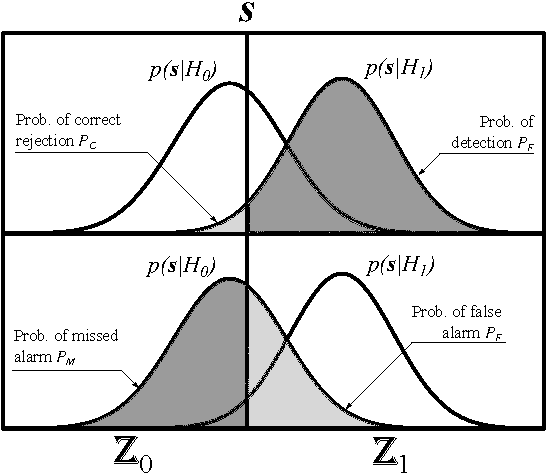
\includegraphics[scale=0.55]{ch3/img/probcurves.pdf}
	\caption{Probability versus decision space}
\end{marginfigure}
\arraymath{
	P(D_0|\hypzero) & = & \int\limits_{\decspacezero}p(\signal|\hypzero)d\signal = 1 - \probfalse \\
	P(D_0|\hypone) & = & \int\limits_{\decspacezero}p(\signal|\hypone)d\signal = \probmiss \\
	P(D_1|\hypzero) & = & \int\limits_{\decspaceone}p(\signal|\hypzero)d\signal = \probfalse \\
	P(D_1|\hypone) & = & \int\limits_{\decspaceone}p(\signal|\hypone)d\signal = 1 - \probmiss
}
where:
\begin{itemize}
\item $\probrej$: represents probability of correct rejection
\item $\probfalse$: represents probability of false alarm
\item $\probmiss$: represents probability of missed alarm
\item $\probdet$: represents probability of detection
\end{itemize}
and, looking at figure \ref{fig:probdetection}, stands the relation:
\arraymath{
	\probdet + \probmiss & = & 1 \\
	\probrej + \probfalse & = & 1
}

Finally, we get the defintion of risk:
\begin{equation}
\begin{array}{rcl} 
R & = & c_{0,0} \braces{1-\probfalse} P(\hypzero) + c_{0,1} \probmiss P(\hypone) + \\ 
  &   &  + c_{1,0} \probfalse P(\hypzero) + c_{1,1} (1-\probmiss) P(\hypone) \\
  & = & P(\hypzero) \braces{c_{0,0} + \probfalse (c_{1,0} - c_{0,0})} + P(\hypone) \braces{c_{1,1} + \probmiss (c_{0,1} - c_{1,1})}
\end{array}
\end{equation}
applying some substitutions:
\arraymath{
	\probmiss & = & \int\limits_{\decspacezero}p(\signal|\hypone)d\signal \\
	\probfalse & = & \int\limits_{\decspaceone}p(\signal|\hypzero)d\signal =  \\
	    & = & 1 - \int\limits_{\decspacezero}p(\signal|\hypzero)d\signal  \\
	1 & = & \int\limits_{\decspacezero}p(\signal|H_j)d\signal + \int\limits_{\decspaceone}p(\signal|H_j)d\signal 
}
and the risk equation:
\begin{equation}
\begin{array}{rcl}
R & = & P(\hypzero) \braces{c_{0,0} + \probfalse (c_{1,0} - c_{0,0})} + P(\hypone) \braces{c_{1,1} + \probmiss (c_{0,1} - c_{1,1})} = \\ 
  & = & P(\hypzero) \braces{c_{0,0} + \braces{1 - \int\limits_{\decspacezero}p(\signal|\hypzero)d\signal} (c_{1,0} - c_{0,0})} + \\ 
  &   &  + P(\hypone) \braces{c_{1,1} + \braces{\int\limits_{\decspacezero}p(\signal|\hypone)d\signal} (c_{0,1} - c_{1,1})} = \\ 
  & = & P(\hypzero) c_{1,0} + P(\hypone) c_{1,1} + \\
  &   & + \int\limits_{\decspacezero} P(\hypone)\braces{c_{0,1} - c_{1,1}} p(\signal|\hypone) - P(\hypzero)\braces{c_{1,0} - c_{0,0}} p(\signal|\hypzero) d\signal
\end{array}
\end{equation}
The first part is constant, to minimize the risk we have to work on the argument of the integral, that depends upon ${\decspacezero}$. Because:
\arraymath{
	P(\hypone)\braces{c_{0,1} - c_{1,1}} p(\signal|\hypone) & \geq & 0 \\
	P(\hypzero)\braces{c_{1,0} - c_{0,0}} p(\signal|\hypzero) & \geq & 0
}
the risk is minimized when:
\begin{equation}
P(\hypone)\braces{c_{0,1} - c_{1,1}} p(\signal|\hypone) < P(\hypzero)\braces{c_{1,0} - c_{0,0}} p(\signal|\hypzero)
\end{equation}
and rearranged as follow
\begin{equation}
\naming{ \dfrac{p(\signal|\hypone)}{p(\signal|\hypzero)} }{\likelihood} < \naming{ \dfrac{P(\hypzero)\braces{c_{1,0} - c_{0,0}}}{P(\hypone)\braces{c_{0,1} - c_{1,1}}} }{\threshold}
\end{equation}
that allow us to define the algorithm \ref{alg:minimumrisk}. Must be noticed:
\begin{itemize}
\item because of the binary nature, the decision rule obtained with the minimization on a single decision, grant the minimization of the risk also on the other decision; thus we could say that the local decision rule minimizes the overall risk
\item the likelihood ratio and threshold define decision regions as follows:
\arraymath{
	\decspacezero &=& \{ \signal\in\decspace \,:\,\likelihood<\threshold \} \\
	\decspaceone &=& \{ \signal\in\decspace \,:\,\likelihood>\threshold \} 
}
and a sample such that $\likelihood=\threshold$ could be assigned arbitrarily to one of the decision region
\item the distributions ${p(\signal|\hypzero)}$ and ${p(\signal|\hypone)}$ should be derived experimentally, something that is not to difficult because of characteristics of our signal
\end{itemize}
\begin{algorithm}[h]
\caption{Minimum risk criterion}
\label{alg:minimumrisk}
\KwData{ $p(\signal|\hypone),\,p(\signal|\hypzero),\,c_{0,0},\,c_{1,0},\,c_{0,1},\,c_{1,1}$ }
\tcc{Define the likelihood ratio}
$\likelihood \leftarrow \dfrac{p(\signal|\hypone)}{p(\signal|\hypzero)} $ \;
\tcc{Define the threshold}
$\threshold \leftarrow \dfrac{P(\hypzero)\braces{c_{1,0} - c_{0,0}}}{P(\hypone)\braces{c_{0,1} - c_{1,1}}}$ \;
\tcc{Binary classification}
\ForAll{$\signal_{in}$}{
	\eIf{$\Lambda(\signal_{in}) \leq \threshold$}{
		\Return{$\signal \in \hypzero$}
	}{
		\Return{$\signal \in \hypone$}
	}
}
\end{algorithm}

\myparagraph{The feature space}
The feature space that could be used are the three signal received from the three orthogonal antennas, plus the position. Te insertion of the position in the feature space is not important for the actual implementation, but could be useful in future, if some computer vision algorithm will be implemented. Algorithms that are able to represent symbolically the dimensions of the avalanche front, in conjunction with slope of the avalanche obtained by the altitude keeping routine, may allow us to define a probability distribution of the possible buried victims, distribution that could be inserted as a priori knowledge in radar detection and searching algorithm.
\FloatBarrier
